
\begin{frame}
{Macierz przekształcenia jednorodnego}
Poniżej znajduje się jedna z interpretacji macierzy przekształcenia jednorodnego.
Przedstawia operację przejścia z układu współrzędnych $0$ do $1$. 
Dzięki temu można przekształcić pozycję obiektu znajdującego się w układzie $0$ i przedstawić jako pozycję względem układu $1$.
Dodatkowo można z niej odczytać położenie i orientację układu $1$ w układzie $0$.
\begin{equation*}
	\prescript{0}{1}T = 
	\begin{bmatrix}
		r_{}11 	& r_{}12	&	r_{}13	& \prescript{0}{1}P_x \\
		r_{}21 	& r_{}22	&	r_{}23	& \prescript{0}{1}P_y \\
		r_{}31 	& r_{}32	& r_{}33	& \prescript{0}{1}P_z \\
		0				&	0				&	0				&	1										\\
	\end{bmatrix}
	\Rightarrow
		\prescript{0}{1}T = 
	 \left[ \begin{array}{c|c}
   \prescript{0}{1}R_{3x3} 	& \prescript{0}{1}P_{3x1} \\
   \midrule
   0_{1x3}									& 1												\\
\end{array}\right]
\end{equation*}
\end{frame}



\begin{frame}
{Drzewo transformacji}
	\begin{itemize}
		\item macierze opisujące przejście między kolejnymi układami odniesienia można mnożyć sekwencyjnie, dzięki czemu relatywnie proste jest przedstawianie układów szeregowych z dużą ilością stawów - drzewo powstaje przez przejście z podstawowego układu (przykładowo świata) przez kolejne układy do docelowego
		\item drzewo transformacji może mieć tylko jeden korzeń, każdy węzeł (układ współrzędnych) tylko jednego rodzica, za to wiele dzieci
	\end{itemize}
	
	
%	\begin{equation*}
%		\prescript{i-1}{i}T = 
%		\begin{bmatrix}
%			c\theta_i	&	-s\theta_i	& 0 &	a_{i-1}	\\
%			s\theta_ic\alpha_{i-1}	&	c\theta_ic\alpha_{i-1}	&	-s\alpha_{i-1}	&	-d_is\alpha_{i-1}	\\
%			s\theta_is\alpha_{i-1}	&	c\theta_is\alpha_{i-1}	&	c\alpha_{i-1}		&	d_ic\alpha_{i-1}\\
%			0	&	0	&	0	&	1	\\
%		\end{bmatrix}
%	\end{equation*}
\end{frame}

\begin{frame}
{Drzewo transformacji robota w zadaniu lokalizacji}
	\begin{columns}
		\begin{column}{0.5\textwidth}
				W kontekście lokalizacji interesująca jest jedynie początkowa część drzewa transformacji opisująca połączenie układu świata z pierwszym układem związanym z robotem.
	Najczęściej między tymi dwoma jest wykonywane przejście przez układ początkowy mapy oraz układ rozpoczęcia odometrii, jeśli jest wykorzystywana.
		\end{column}
		\begin{column}{0.5\textwidth}  %%<--- here
			\begin{figure}
				\begin{center}
					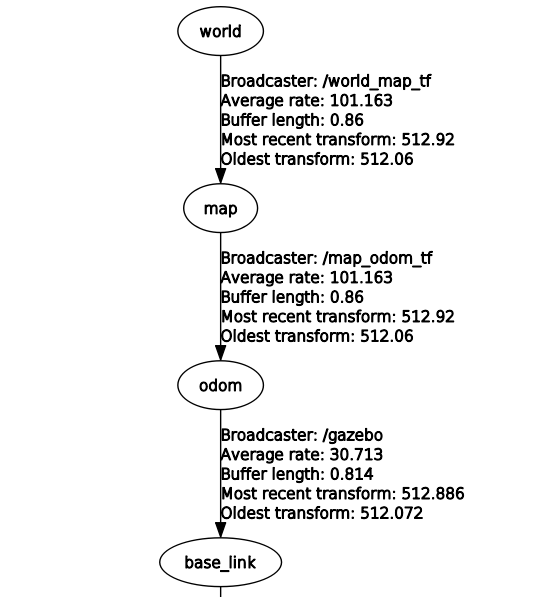
\includegraphics[height=0.6\textheight]{img/velma_tf.png} 
					\caption{początek drzewa transformacji po uruchomieniu symulacji robota}
				\end{center}
			\end{figure}
		\end{column}
	\end{columns}
\end{frame}

\begin{frame}
{Odometria}
	\begin{columns}
		\begin{column}{0.45\textwidth}
			\begin{itemize}
				\item metoda lokalizacji zliczeniowej
				\item obliczenie pozycji robota na podstawie oszacowanej prędkości, kierunku i czasu ruchu
				\item względnie proste zadanie obliczeniowo, ale generuje systematycznie akumulowane błędy
			\end{itemize}
		\end{column}
		\begin{column}{0.55\textwidth}  %%<--- here
			\begin{figure}
				\begin{center}
					\includegraphics[page={180},clip, trim=8cm 1.5cm 3cm 18cm, scale=0.6]{pdf/2017_Book_RoboticsVisionAndControl.pdf}
					\hspace*{15pt}\hbox{\scriptsize{Źródło:\thinspace{\footnotesize{\itshape{Robotics Vision and Control \cite{robotics_vision}}}}}}
					\caption{Błędy odometrii. Niebieska droga oznacza rzeczywistą ścieżkę, czerwona ścieżka obliczoną }
				\end{center}
			\end{figure}
		\end{column}
	\end{columns}
\end{frame}

\begin{frame}
{Lokalizacja z wykorzystaniem znaczników}
	\begin{itemize}
		\item wykorzystuje punkty o znanym położeniu względem początkowego układu współrzędnych mapy, które robot jest w stanie rozróżnić i zidentyfikować
		\item mierząc pozycję robota względem punktów można obliczyć jego pozycję względem początkowego układu mapy
		\item ta metoda również zwraca pozycję z pewnym błędem z powodu niepewności zmierzonej pozycji znaczników, jak i niepewności pomiarowych pozycji ich względem robota, lecz ten błąd jest ograniczony, im lepiej umieszczone znaczniki, tym mniejszy
	\end{itemize}
\end{frame}

\begin{frame}
{Lokalizacja z wykorzystaniem systemu LiDAR}
	\begin{itemize}
		\item problem podobny do poprzedniego, lecz bez rozpoznawania znaczników
		\item wykorzystanie algorytmu ICP (iterative closed point) do dopasowania aktualnego skanu robota do stworzonej uprzednio mapy
		\item niezależność od specjalnych znaczników, lecz większy nakład obliczeniowy
		\item w przypadku gdy zbudowana mapa składa się z podobnych fragmentów może się okazać, że algorytm zawiedzie (przykładowo jazda długim korytarzem bez elementów szczególnych)
	\end{itemize}
\end{frame}

